\subsection{K-anonymat} 

Le K-anonymisation est une technique d’anonymisation qui empêche qu’une personne ne soit isolée dans un jeu de données. Elle permet ainsi de regrouper un individu avec au moins K autres individus, de sorte qu’il y ait moins de chance de retrouver l’individu en question. En d’autres mots, on généralise certains attributs de telle manière à ce que ces derniers soient identiques pour un groupe de K individus [4;11]. 

\paragraph{Etapes de la k-anonymisation:} 
\begin{itemize}
    \item  Déterminer les ensembles d’attributs qui peuvent être utilisés pour croiser les données anonymes avec des données identifiants. 

    \item Réduire le niveau de détail des données de telle sorte qu’il y ait au moins k individus qui ont la même valeur de quasi-identifiants. 
\end{itemize}

%% ajout d'exemple
\begin{figure}[!h]
    \centering
    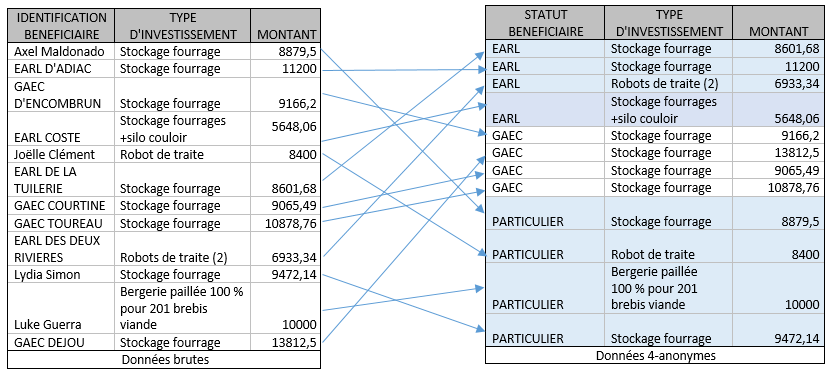
\includegraphics[width=1\textwidth]{images/anonymisation/k_anonym_image1.png}
    \caption{Exemple d'une k-anonymisation : données 4-anonymes}
    \label{Exemple d'une k-anonymisation : données 4-anonymes}
\end{figure}


\paragraph{Evaluation du k-anonymat:}  
\begin{itemize}
    \item \textbf{Individualisation :} étant données les classes d’équivalence, nous savons qu’au moins k individus partagent certains attributs dans le jeu de données. Il ne devrait plus être possible d’isoler un individu dans un groupe de k autres individus. 

    \item \textbf{Corrélation:} il est possible de relier les enregistrements par groupe de k-individus. Au sein d’un même groupe, la probabilité que deux enregistrements correspondent à un individu est de 1/k. 

    \item \textbf{Inférence:} si tous les k individus d’une classe d’équivalence ont la même valeur pour un attribut donné et que cette information est sensible, il suffit de connaître à quelle classe d’équivalence appartient un individu pour déduire sa données sensible. 
\end{itemize}
 
Alors que k-anonymat protège contre la divulgation d'identité, il n'offre pas une protection suffisante contre la divulgation d'attributs. Cela a été reconnu par plusieurs auteurs[13], [14]. Deux attaques ont été identifiées dans: attaque d'homogénéité et l'attaque de connaissances de fond[14]. 